\documentclass{standalone}
\usepackage{tikz}
\usetikzlibrary{decorations.pathreplacing}
\usepackage{amsfonts}

\begin{document}
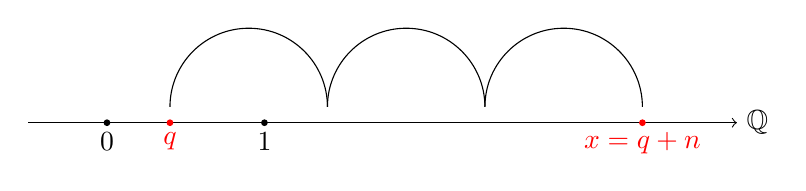
\begin{tikzpicture}
% Draw the real line
  \draw[->] (-1,0) -- (8,0) node[right] {$\mathbb{Q}$};
  
  % Draw the point 'x' and '0'
   \filldraw (0,0) circle (1pt) node[below] {$0$};
  \filldraw[red] (0.8,0) circle (1pt) node[below] {$q$};
    \filldraw (2,0) circle (1pt) node[below] {$1$};
    
   
   % \filldraw (2.8,0) circle (1pt) node[below] {$\tilde{t} + T$};
     
   %  \filldraw (4.8,0) circle (1pt) node[below] {$\tilde{t} + 2T$};
     
      \filldraw[red] (6.8,0) circle (1pt) node[below] {$x = q + n$};


  
 
\draw (2.8,0.2) arc (0:180:1);
\draw (4.8,0.2) arc (0:180:1);
\draw (6.8,0.2) arc (0:180:1);
  
  
  \end{tikzpicture}
\end{document}